%%%%%%%%%%%%%%%%%%%%%%%%%%%%%%%%%%%%%%%%%
% Beamer Presentation
% LaTeX Template
% Version 1.0 (10/11/12)
%
% This template has been downloaded from:
% http://www.LaTeXTemplates.com
%
% License:
% CC BY-NC-SA 3.0 (http://creativecommons.org/licenses/by-nc-sa/3.0/)
%
%%%%%%%%%%%%%%%%%%%%%%%%%%%%%%%%%%%%%%%%%

%----------------------------------------------------------------------------------------
%	PACKAGES AND THEMES
%----------------------------------------------------------------------------------------

\documentclass{beamer}

\mode<presentation> {

% The Beamer class comes with a number of default slide themes
% which change the colors and layouts of slides. Below this is a list
% of all the themes, uncomment each in turn to see what they look like.

%\usetheme{default}
%\usetheme{AnnArbor}
%\usetheme{Antibes}
%\usetheme{Bergen}
%\usetheme{Berkeley}
%\usetheme{Berlin}
%\usetheme{Boadilla}
%\usetheme{CambridgeUS}
%\usetheme{Copenhagen}
%\usetheme{Darmstadt}
%\usetheme{Dresden}
%\usetheme{Frankfurt}
%\usetheme{Goettingen}
%\usetheme{Hannover}
%\usetheme{Ilmenau}
%\usetheme{JuanLesPins}
%\usetheme{Luebeck}
\usetheme{Madrid}
%\usetheme{Malmoe}
%\usetheme{Marburg}
%\usetheme{Montpellier}
%\usetheme{PaloAlto}
%\usetheme{Pittsburgh}
%\usetheme{Rochester}
%\usetheme{Singapore}
%\usetheme{Szeged}
%\usetheme{Warsaw}

% As well as themes, the Beamer class has a number of color themes
% for any slide theme. Uncomment each of these in turn to see how it
% changes the colors of your current slide theme.

%\usecolortheme{albatross}
%\usecolortheme{beaver}
%\usecolortheme{beetle}
%\usecolortheme{crane}
%\usecolortheme{dolphin}
%\usecolortheme{dove}
%\usecolortheme{fly}
%\usecolortheme{lily}
%\usecolortheme{orchid}
%\usecolortheme{rose}
%\usecolortheme{seagull}
%\usecolortheme{seahorse}
%\usecolortheme{whale}
%\usecolortheme{wolverine}

%\setbeamertemplate{footline} % To remove the footer line in all slides uncomment this line
%\setbeamertemplate{footline}[page number] % To replace the footer line in all slides with a simple slide count uncomment this line

%\setbeamertemplate{navigation symbols}{} % To remove the navigation symbols from the bottom of all slides uncomment this line
\def\mathfamilydefault{\rmdefault}
%\setbeamertemplate{navigation symbols}{} % To remove the navigation symbols from the bottom of all slides uncomment this line
\logo{
\includegraphics[height=1.1cm]{logo.png}}
\setbeamertemplate{navigation symbols}{} % To remove the navigation symbols from the bottom of all slides uncomment this line
}

\usepackage{graphicx} % Allows including images
\usepackage{subfigure}
\usepackage{booktabs} % Allows the use of \toprule, \midrule and \bottomrule in tables
\usepackage{listings}
\lstset{
	numbers=left, 
	numberstyle= \tiny, 
	keywordstyle= \color{ blue!70},
	commentstyle= \color{red!50!green!50!blue!50}, 
	frame=shadowbox, % 阴影效果
	rulesepcolor= \color{ red!20!green!20!blue!20} ,
	escapeinside=``, % 英文分号中可写入中文
	xleftmargin=2em,xrightmargin=2em, aboveskip=1em,
	framexleftmargin=2em
} 
\lstset{language=python}
\lstset{breaklines}
\usepackage{xcolor}

%----------------------------------------------------------------------------------------
%	TITLE PAGE
%----------------------------------------------------------------------------------------

\title[Quantum Optics with Python]{Quantum Optics with Python: \\
	Lecture2:Qutip and Quasi-probability theory} % The short title appears at the bottom of every slide, the full title is only on the title page

\author{Cai Jiaqi} % Your name
\institute[HUST] % Your institution as it will appear on the bottom of every slide, may be shorthand to save space
{
Huazhong University of Science and Technology \\ % Your institution for the title page
\medskip
\textit{caidish@hust.edu.cn} % Your email address
}
\date{\today} % Date, can be changed to a custom date

\begin{document}

\begin{frame}
\titlepage % Print the title page as the first slide
\end{frame}

\begin{frame}
\frametitle{Overview} % Table of contents slide, comment this block out to remove it
\tableofcontents % Throughout your presentation, if you choose to use \section{} and \subsection{} commands, these will automatically be printed on this slide as an overview of your presentation
\end{frame}

%----------------------------------------------------------------------------------------
%	PRESENTATION SLIDES
%----------------------------------------------------------------------------------------

%------------------------------------------------
\section{An Introduction to Qutip}
\begin{frame}{What is Qutip?}
\begin{center}
	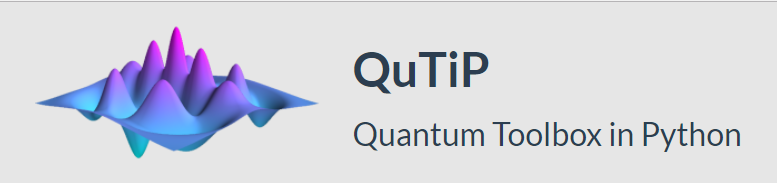
\includegraphics[width=0.7\linewidth]{screenshot001}
\end{center}
\begin{block}{Qutip}
	Quantum Toolbox in Python.URL:http://qutip.org/ \\
	Cite them with  Comp. Phys. Comm. 184, 1234 (2013) or  Comp. Phys. Comm. 183, 1760 (2012)!
\end{block}
\end{frame}

\begin{frame}{Why I choose Qutip?}
\begin{itemize}
	\item Free
	\item Easy
	\item Partially Fast
	\item Interactive
	\item Universal and Scalable
\end{itemize}
\end{frame}

\begin{frame}{How Many People are Using Qutip?}
Many people in the community of Quantum optics and related subjects are now using Qutip. Qutip helps to generate beautiful figure and simulation results of many high-quality papers.

In 2016,the Unique Visitors of qutip.org is larger than 25,473.
\end{frame}

\subsection{Installation and Some Dos and Don'ts}
\begin{frame}{Windows}
Qutip is first developed on Unix and tested mostly on Linux. But thanks to the portability of Python language, Windows users can also use Qutip as you like.

The recommended installation steps are:

\begin{itemize}
	\item Install MSVC++ 2015 or VS2015.Notice: The default installation of VS2015 DON'T contain MSVC++ any more! You need to change the default to a manual one.
	\item Install Anaconda. For CERNET user, I highly recommend you to download the distribution from Tsinghua Opensource Mirror
	\item Pip install Qutip.
	\item enjoy it!
\end{itemize}

\end{frame}

\begin{frame}{Linux and macOs}
\begin{itemize}
	\item Install gcc.\\Note: Ubuntu: sudo wget build-essentials. Mac: brew install gcc.
	\item Install Anaconda.
	\item pip install Qutip.
	\item enjoy it!
\end{itemize}
	
\end{frame}

\subsection{Finite Hilbert Space!}
\begin{frame}{Hilbert Space}
A computer can only hold a finite representation of Hilbert space. For analytic method, the Fock state can be represented as:
\[\left\langle {m}
\mathrel{\left | {\vphantom {m n}}
	\right. \kern-\nulldelimiterspace}
{n} \right\rangle  = {\delta _{mn}},\left| n \right\rangle  = A{\left( {{a^\dag }} \right)^n}\left| 0 \right\rangle \]
However, this Fock state cannot be stored conveniently by a computer. 

In qutip, we often set an upper bound of Hilbert space, e.g. $n$ . Then, states are $1\times n$ vectors and operators are $n \times n$ matrix.

To generate many-body Hamiltonian, we should construct a total space from the tensor product(e.g,kronecker product) of two spaces: 
\[{H^{total}} = {H^{\left( 1 \right)}} \otimes {H^{\left( 2 \right)}}\]
\end{frame}

\subsection{States and Operators}
\begin{frame}{States and Operators in Qutip}
static function:basis(), create(), destroy(), tensor(),mesolve().....

Qobj class, properties: 
dims,
shape,
type,
data

some selected function:*,dag(),eigenenergies(),eigenstates,
\end{frame}
\begin{lstlisting}
d = 5
#the dimension of the Hilbert space
g = basis(d,0)
e1 = basis(d,1)
e2 = basis(d,2)
print(g)
print(e1)
print(e2)

a=destroy(d)
a_dag = create(d)
e1 = a_dag*g
e2 = (a_dag * a_dag * g).unit()
print(g)
print(e1)
print(e2)
\end{lstlisting}\frametitle{States and Operators in Qutip}
\subsection{Solving Equation of Quantum System by Qutip}
\begin{frame}{Master Equation Solver}
\begin{block}{Unitary Evolution}
	\[\psi \left( t \right) = U\left( {t,0} \right)\psi \left( 0 \right)\]
	mesolve(H,psi0,times,[],[(exp)])
\end{block}
\begin{block}{Non-unitary Evolution}
\[\frac{d}{{dt}}\rho \left( t \right) =  - \frac{i}{\hbar }\left[ {H\left( t \right),\rho \left( t \right)} \right] + \sum\limits_n {\frac{1}{2}\left[ {2{C_n}\rho \left( t \right)C_n^\dag  - \rho \left( t \right)C_n^\dag {C_n} - C_n^\dag {C_n}\rho \left( t \right)} \right]} \]

mesolve(H,psi0,times,[c\_ops\_list],[(exp)])
\end{block}

\end{frame}
\begin{frame}{Spin Model and Spin with Dissipation}
The Hamiltonian of a spin in x-direction is read as:$H = {\omega _z}{\sigma _x}$. The dynamic evolution of this system can be obtained by qutip.

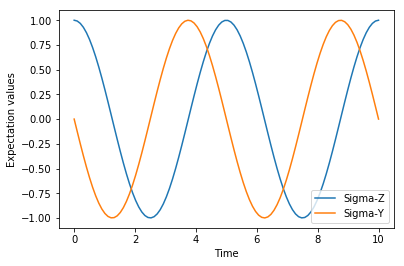
\includegraphics[width=0.5\linewidth]{2}
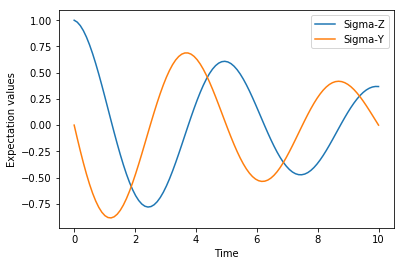
\includegraphics[width=0.5\linewidth]{3}


\end{frame}

\begin{lstlisting}
H = 2 * np.pi * 0.1 * sigmax()
psi0 = basis(2, 0)
times = np.linspace(0.0, 10.0, 20)
result = mesolve(H, psi0, times, [], [sigmaz(),sigmay()])
fig, ax = plt.subplots()
ax.plot(result.times, result.expect[0]);
ax.plot(result.times, result.expect[1]);
ax.set_xlabel('Time');
ax.set_ylabel('Expectation values');
ax.legend(("Sigma-Z", "Sigma-Y"));
plt.show()
\end{lstlisting}
\newpage
\begin{lstlisting}
H = 2 * np.pi * 0.1 * sigmax()
psi0 = basis(2, 0)
times = np.linspace(0.0, 10.0, 20)
result = mesolve(H, psi0, times, [np.sqrt(0.05)*sigmax()], [sigmaz(),sigmay()])
fig, ax = plt.subplots()
ax.plot(result.times, result.expect[0]);
ax.plot(result.times, result.expect[1]);
ax.set_xlabel('Time');
ax.set_ylabel('Expectation values');
ax.legend(("Sigma-Z", "Sigma-Y"));
plt.show()
\end{lstlisting}
\begin{frame}{Mento Carlo Solver}
\[\begin{gathered}
{H_{eff}} = {H_{sys}} - \frac{i}{2}\sum\limits_i {C_n^\dag {C_n}}  \hfill \\
\psi \left( {t + dt} \right) = {C_n}\psi \left( t \right)/\sqrt {\left\langle {C_n^\dag {C_n}} \right\rangle }  \hfill \\ 
\end{gathered} \]
usage:mesolve(H,psi0,times,[c\_ops\_list],[(exp)])
\end{frame}
\begin{frame}{Steady State Solver}
\[\frac{{d{\rho _{ss}}}}{{dt}} = L{\rho _{ss}} = 0\]

usage:steadystates(H,c\_ops)
\end{frame}
\begin{frame}{Example:Optomechanical System}
\begin{figure}
	\centering
	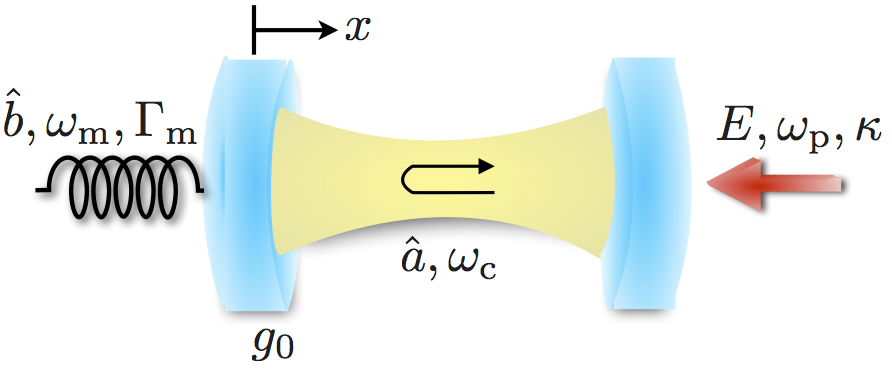
\includegraphics[width=0.5\linewidth]{download}
	\label{fig:download}
\end{figure}
The optomechanical Hamiltonian arises from the radiation pressure interaction of light in an optical cavity where one of the cavity mirrors is mechanically compliant:
$$\frac{\hat{H}}{\hbar}=-\Delta\hat{a}^{+}\hat{a}+\omega_{m}\hat{b}^{+}\hat{b}+g_{0}(\hat{b}+\hat{b}^{+})\hat{a}^{+}\hat{a}+E\left(\hat{a}+\hat{a}^{+}\right)$$
Where $\Delta$is the detuning between pump($\omega_{p}$) and cavity($\omega_c$), $\omega_{m}$ is frequency of the oscillator. $g_0$ is the single-photon-phonon coupling strength and $E$ is the amplitude of the pump mode.

\end{frame}
\begin{frame}{Example:Optomechanical System}
To obtain the dynamic evolution of the system , we'll follow the steps below:
\begin{itemize}
	\item Set system parameter
	\item Build Hamiltonian and collapse operators
	\item Solve master equation
	\item Run steady state Solver
	\item Visualize the result
\end{itemize}
\end{frame}

\begin{frame}{Example:Optomechanical System}
	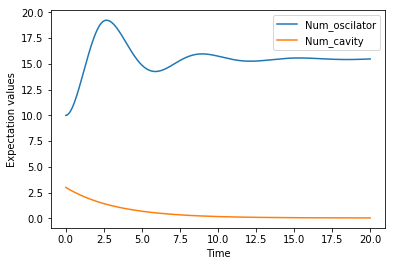
\includegraphics[width=0.5\linewidth]{4}
	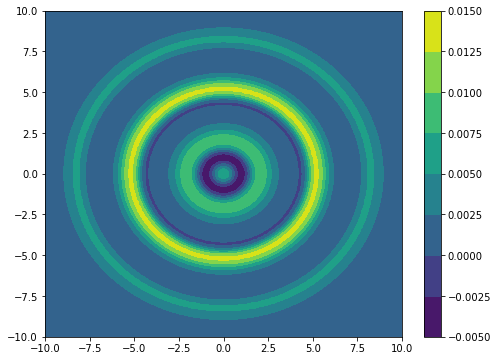
\includegraphics[width=0.5\linewidth]{5}

\end{frame}

\begin{lstlisting}
# System Parameters (in units of wm)
#-----------------------------------
Nc = 10                      # Number of cavity states
Nm = 80                     # Number of mech states
kappa = 0.3                 # Cavity damping rate
E = 0.1                     # Driving Amplitude         
g0 = 2.4*kappa              # Coupling strength
Qm = 1e4                    # Mech quality factor
gamma = 1/Qm                # Mech damping rate
n_th = 1                    # Mech bath temperature
delta = -0.43               # Detuning

# Operators
#----------
a = tensor(destroy(Nc), qeye(Nm))
b = tensor(qeye(Nc), destroy(Nm))
num_b = b.dag()*b
num_a = a.dag()*a
psi0=tensor(basis(Nc,5),basis(Nm,10))
ro0 = psi0*psi0.dag()
# Hamiltonian
#------------
H = -delta*(num_a)+num_b+g0*(b.dag()+b)*num_a+E*(a.dag()+a)

# Collapse operators
#-------------------
cc = np.sqrt(kappa)*a
cm = np.sqrt(gamma*(1.0 + n_th))*b
cp = np.sqrt(gamma*n_th)*b.dag()
c_ops = [cc,cm,cp]

t_list = np.linspace(0,20,1000)
result = mesolve(H,ro0,times,c_ops,[num_b,num_a])
\end{lstlisting}
\section{An Introduction to Quasi-probability Theory}
\subsection{Motivation}
\begin{frame}{Motivation}
\begin{block}{Classical version of fluctuating of complex E(t)}
	\[\left\langle {{E^*}\left( {{r_1},t} \right)E\left( {{r_2},t} \right)} \right\rangle  = \int {{E^*}\left( {{r_1},t} \right)E\left( {{r_2},t} \right)P\left( {E,{E^*},t} \right){d^2}E} \]
\end{block}
Q: Can we construct a similar description for quantum field fluctuations?

A:The quasi-probability theory in coherent state representation!

But: \centering{\textbf{???$a^{\dagger}$ and $a$ are not commute???}}

\begin{itemize}
	\item Normal ordering ${a^\dag }a$-----\emph{P-representation}
	\item Anti-normal ordering $a{a^\dag }$-----\emph{Q-representation}
	\item Symmetric ordering $\left( {a{a^\dag } + {a^\dag }a} \right)/2$-----\emph{Wigner function}
\end{itemize}

\end{frame}


\subsection{P-representation}
\begin{frame}{P-representation: Theoretical Case}
We want to expand any operator of the light field with probability distribution, Which means:
\[\left\langle {O\left( {a,{a^\dag }} \right)} \right\rangle  = \int {{d^2}\alpha P\left( {\alpha ,{\alpha ^*}} \right)O\left( {\alpha ,{\alpha ^ * }} \right)} \]

Basically, any operator can be expanded in a normal ordering:
\[\delta \left( {{\alpha ^*} - {a^\dag }} \right)\delta \left( {\alpha  - a} \right) = \frac{1}{{{\pi ^2}}}\int {{d^2}\beta \left[ {{e^{ - \beta \left( {{\alpha ^*} - {a^\dag }} \right)}}{e^{\beta \left( {\alpha  - a} \right)}}} \right]} \]
Then, take the expectation value of the operator:
\[\left\langle {O\left( {a,{a^\dag }} \right)} \right\rangle  = Tr\left[ {\rho O} \right] = \sum\limits_n {\sum\limits_m {{c_{nm}}Tr\left[ {\rho {{\left( {{a^\dag }} \right)}^n}{a^m}} \right]} } \]
Define an operator:
\[\delta \left( {{\alpha ^*} - {a^\dag }} \right)\delta \left( {\alpha  - a} \right) = \frac{1}{{{\pi ^2}}}\int {{d^2}\beta \left[ {{e^{ - \beta \left( {{\alpha ^*} - {a^\dag }} \right)}}{e^{\beta \left( {\alpha  - a} \right)}}} \right]} \]


\end{frame}

\begin{frame}{P-representation: Theoretical Case}
Then, the expectation can be written as:
\[\left\langle O \right\rangle  = \int {{d^2}\alpha \sum\limits_n {\sum\limits_m {{c_{nm}}Tr\left[ {\rho \delta \left( {{\alpha ^*} - {a^\dag }} \right)\delta \left( {\alpha  - a} \right)} \right]{{\left( {{\alpha ^*}} \right)}^n}{\alpha ^m}} } } \]

So:
\[P\left( {\alpha ,{\alpha ^*}} \right) \equiv Tr\left[ {\rho \delta \left( {{\alpha ^*} - {a^\dag }} \right)\delta \left( {\alpha  - a} \right)} \right]\]

A convenient way to calculate P-function is take the Fourier inverse of anti-diagonal matrix element of $\rho$ (exercise):
\[P\left( {\alpha ,{\alpha ^*}} \right) = {\mathfrak{F}_{{x_\beta },{y_\beta } \to {x_\alpha },{y_\alpha }}}\left[ {\left\langle { - \beta } \right|\rho \left| \beta  \right\rangle {e^{{{\left| \beta  \right|}^2}}}} \right]\]

\end{frame}

\begin{frame}{P-representation:Quantum Fock state}
Last time, it is mentioned that Fock state is a quantum state of light. Here comes the reason:

$\rho  = \left| n \right\rangle \left\langle n \right|$ is the density matrix of a Fock state, and 
\[\left\langle { - \beta } \right|\rho \left| \beta  \right\rangle  = \exp \left( { - {{\left| \beta  \right|}^2}} \right)\frac{{{{\left( { - 1} \right)}^n}{{\left| \beta  \right|}^{2n}}}}{{n!}}\]

It then follows that:
\[\begin{gathered}
P\left( {\alpha ,{\alpha ^*}} \right) = \frac{{{e^{{{\left| \alpha  \right|}^2}}}}}{{{\pi ^2}}}\frac{{{{\left( { - 1} \right)}^n}}}{{n!}}\int {{d^2}\beta } \left[ {{{\left| \beta  \right|}^{2n}}{e^{ - \beta {\alpha ^*} + {\beta ^*}\alpha }}} \right] \hfill \\
= \frac{{{e^{{{\left| \alpha  \right|}^2}}}}}{{{\pi ^2}}}\frac{{{{\left( { - 1} \right)}^n}}}{{n!}}\frac{{{\partial ^{2n}}}}{{\partial {\alpha ^n}\partial {\alpha ^{*n}}}}\int {{d^2}\beta } \left[ {{e^{ - \beta {\alpha ^*} + {\beta ^*}\alpha }}} \right] \hfill \\
= \frac{{{e^{{{\left| \alpha  \right|}^2}}}}}{{{\pi ^2}}}\frac{{{{\left( { - 1} \right)}^n}}}{{n!}}\frac{{{\partial ^{2n}}}}{{\partial {\alpha ^n}\partial {\alpha ^{*n}}}}{\delta ^2}\left( {\alpha ,{\alpha ^*}} \right) \hfill \\ 
\end{gathered} \]

Which turns out to be \textbf{negative}. In a classical version of distribution theory, probability is required to be nonnegative! These whose $P(\alpha,\alpha^{\star})$ is negative for some value are called non-classical. 
\end{frame}

\subsection{Q-representation}
\begin{frame}{Q-representation: Theoretical Case}
The definition of Q-representation is:
\[\begin{gathered}
Q\left( {\alpha ,{\alpha ^*}} \right) = Tr\left[ {\rho \delta \left( {\alpha  - a} \right)\delta \left( {{\alpha ^*} - {a^\dag }} \right)} \right] \hfill \\
Q\left( {\alpha ,{\alpha ^*}} \right) = \frac{1}{\pi }\left\langle \alpha  \right|\rho \left| \alpha  \right\rangle  \hfill \\ 
\end{gathered} \]
It then follows that(exercise):
\[\left\langle {O\left( {a,{a^\dag }} \right)} \right\rangle  = \int {Q\left( {\alpha ,{\alpha ^*}} \right)O\left( {\alpha ,{\alpha ^*}} \right)} {d^2}\alpha \]
And $Q\left( {\alpha ,{\alpha ^*}}\right)$ is nonnegative and bounded(exercise):
\[0 \leqslant Q\left( {\alpha ,{\alpha ^*}} \right) \leqslant \frac{1}{\pi }\]
\end{frame}
\subsection{Wigner-function}
\begin{frame}{Wigner Distribution: Theoretical Case}
Note that $P\&Q$ can be written in terms of \textbf{characteristic functions}. So:

\[\begin{gathered}
P\left( {\alpha ,{\alpha ^*}} \right) = \frac{1}{{{\pi ^2}}}\int {{d^2}\beta {e^{ - i\beta {\alpha ^*} - i{\beta ^*}\alpha }}{C^p}\left( {\beta ,{\beta ^*}} \right)}  \hfill \\
{C^p}\left( {\beta ,{\beta ^*}} \right) = Tr\left[ {{e^{i\beta {a^\dag }}}{e^{i{\beta ^*}a}}\rho } \right] \hfill \\
Q\left( {\alpha ,{\alpha ^*}} \right) = \frac{1}{{{\pi ^2}}}\int {{d^2}\beta {e^{ - i\beta {\alpha ^*} - i{\beta ^*}\alpha }}{C^Q}\left( {\beta ,{\beta ^*}} \right)}  \hfill \\
{C^Q}\left( {\beta ,{\beta ^*}} \right) = Tr\left[ {{e^{i{\beta ^*}a}}{e^{i\beta {a^\dag }}}\rho } \right] \hfill \\ 
\end{gathered} \]

Wigner and Weyl introduced Wigner function, which is defined as:
\[\begin{gathered}
W\left( {\alpha ,{\alpha ^*}} \right) = \frac{1}{{{\pi ^2}}}\int {{d^2}\beta {e^{ - \beta {\alpha ^*} - i{\beta ^*}\alpha }}{C^W}\left( {\beta ,{\beta ^*}} \right)}  \hfill \\
{C^W}\left( {\beta ,{\beta ^*}} \right) = Tr\left[ {{e^{i{\beta ^*}a + i\beta {a^\dag }}}} \right] \hfill \\ 
\end{gathered} \]
Among three types of quasi-distribution, Wigner function is used mostly because it serves as a phase diagram of a quantum state.
\end{frame}

\begin{frame}{Wigner Distribution:Vacuum state, Coherent state and squeezed state}

\begin{figure}
	\centering
	\subfigure[Vacuum state displacing to a cohrent state]{
		\begin{minipage}[b]{0.4\textwidth}
			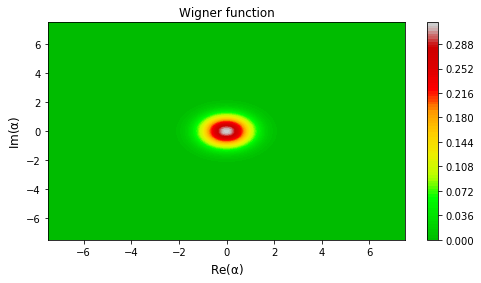
\includegraphics[width=1\textwidth]{6} \\
			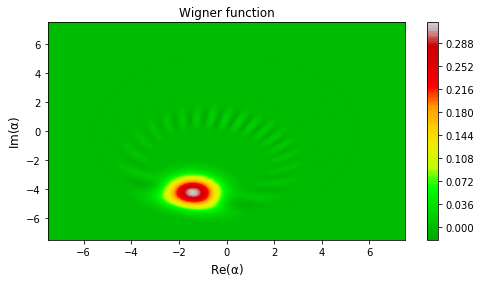
\includegraphics[width=1\textwidth]{8}
		\end{minipage}
	}
	\subfigure[Cohrent state squezing to a squezeed state]{
		\begin{minipage}[b]{0.4\textwidth}
			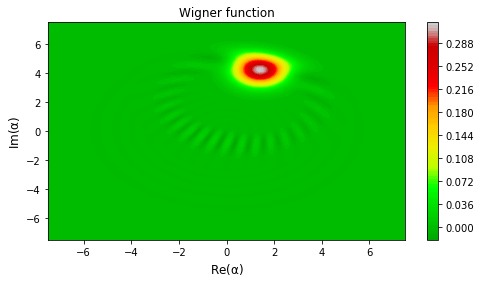
\includegraphics[width=1\textwidth]{7} \\
			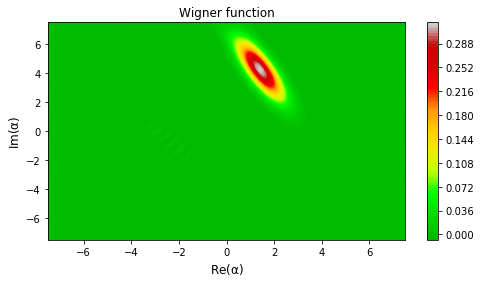
\includegraphics[width=1\textwidth]{9}
		\end{minipage}
	}
\end{figure}
\end{frame}
\begin{lstlisting}
N = 50
vac = basis(N,0)
rho_vac = vac*vac.dag()
rho_coh1 = coherent_dm(N,1+3j)
rho_coh2 = coherent_dm(N,-1-3j)
plot_wigner(rho_vac,colorbar=True,cmap='spectral')
plot_wigner(rho_coh1,colorbar=True,cmap='spectral')
plot_wigner(rho_coh2,colorbar=True,cmap='spectral')
vac = basis(N,0)
d = displace(N,1+3j)
s = squeeze(N,0.25+0.25j)
psi = s*d*vac
rho = psi*psi.dag()
plot_wigner(rho,colorbar=True,cmap='spectral')
\end{lstlisting}
\section{Some Examples and Exercise}
\subsection{Cat State(Demo)}
\begin{frame}{Cat State(Demo)}
Consider a so-called Schrodinger-cat state
\[\left| \psi  \right\rangle  = \left| \alpha  \right\rangle  + \left| { - \alpha } \right\rangle \]
where $\left| \alpha  \right\rangle $ is a coherent state. (a) Find the normalization constant N. (b)
What is the photon distribution function and wigner function?
\end{frame}
\begin{frame}{Cat State(Demo)}
\begin{center}
	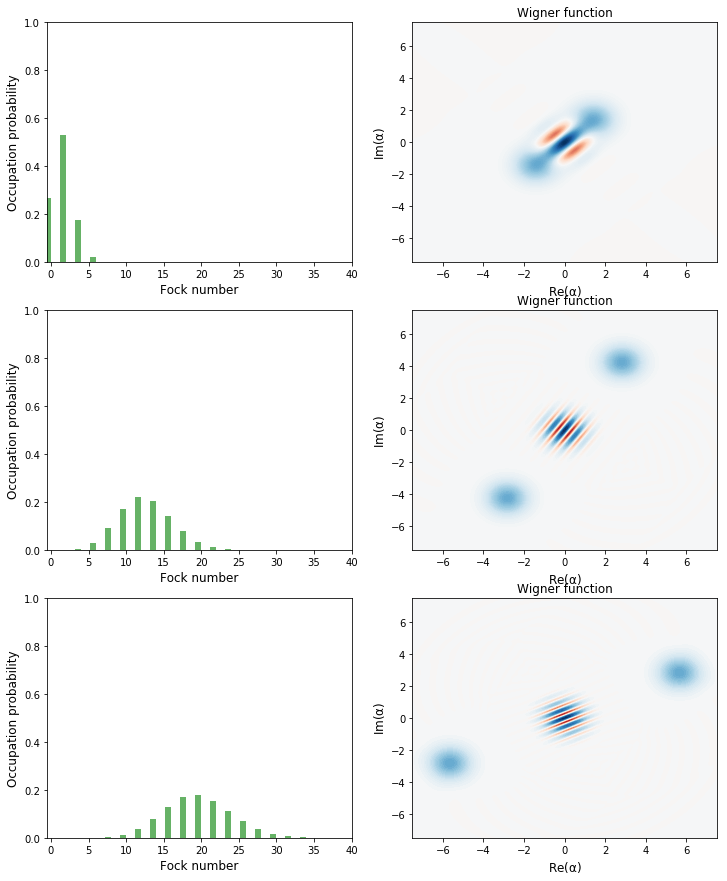
\includegraphics[width=0.4\linewidth]{screenshot007}
\end{center}


\end{frame}
\subsection{Kerr Effect to Create Cat State(Exercise)}
\begin{frame}{Kerr Effect to create Cat state(exercise)}
The effective Hamiltonian will result in Cat state from an initial coherent state:
\[H = \frac{1}{2}\chi {a^\dag }{a^\dag }aa = \frac{1}{2}\chi n\left( {n - 1} \right)\]
Test and verify this by numerical simulations.
\begin{figure}
	\centering
	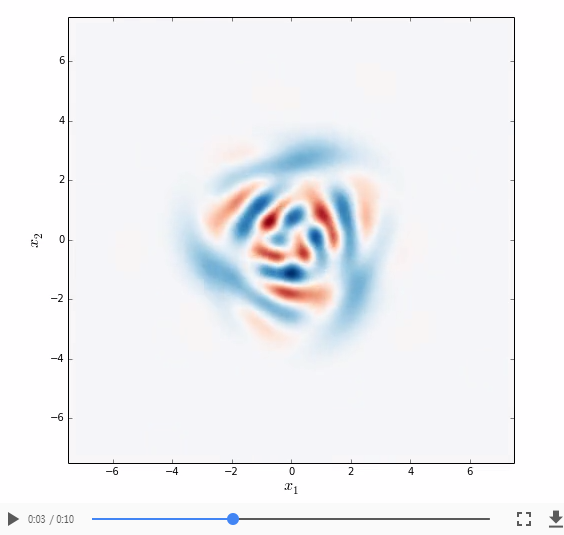
\includegraphics[width=0.3\linewidth]{screenshot002}
	\caption{See:\emph{Kirchmair, G., Vlastakis, B., Leghtas, Z., Nigg, S. E., Paik, H., Ginossar, E., … Schoelkopf, R. J. (2012). Observation of quantum state collapse and revival due to the single-photon Kerr effect. Nature, 495(7440), 205–209. https://doi.org/10.1038/nature11902} for details}
	\label{fig:screenshot002}
\end{figure}
see:
\end{frame}

\end{document} 